\section{Explainability of Neural Networks}
Neural networks have become one of major machine learning algorithms used in many applications, for example computer vision and medicine. Despite those achievements, they are still considered as a blackbox process that is  difficult to interpret its results or find evidences that the networks use to make such accurate decisions for further analyses.


%\begin{figure}
%  \centering
%  \begin{minipage}{\textwidth}
%  
%			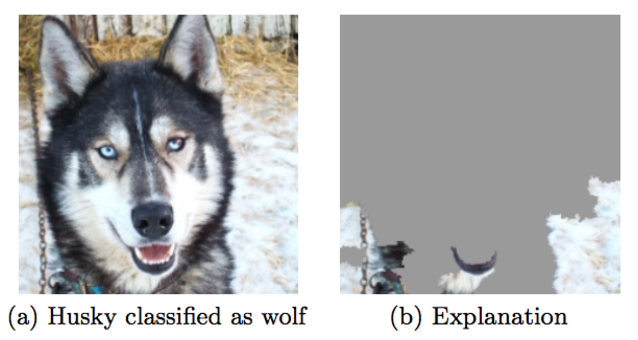
\includegraphics[width=0.6\textwidth]{sketch/husky_explanation}
%
%    \caption[Compact Routing Example]%
%    {Compact Routing\footnote{something} Example}
%  \end{minipage}
%\end{figure}
%


 \begin{figure}[!hbt]
	 		\centering
			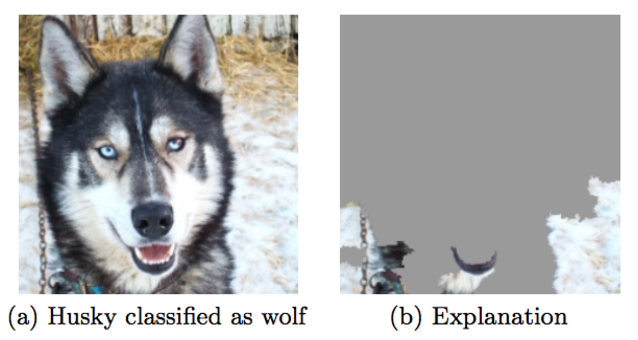
\includegraphics[width=0.6\textwidth]{sketch/husky_explanation}
			\caption{A classifier classifies ``husky" as ``wolf" because of the snow background.}
			  \small{ Source : \cite{RibeiroWhyShouldTrust2016} }
			\label{fig:husky_explanation}
\end{figure}
%\footnotetext{}


Moreover, it is always important to verify whether trained neural networks properly utilize data or what information it uses to make decisions. Literatures refer this functional inspection as ``Explainability'' or ``Interpretability". \cite{BachAnalyzingclassifiersFisher2016, RibeiroWhyShouldTrust2016} demonstrated that there are cases that some neural networks exploit artifacts in the data to make decisions. \addfigure{\ref{fig:husky_explanation}} is such an example. This discoveries emphasize the importance of having explainable neural networks, not to mention the fact that nowadays neural networks have involved in several aspects that human's life is involved, such as medicine or self-driving car. Therefore, having more explainable models is necessary.

\subsection{Global and Local Explanation}
Formally, interpreting neural networks can analyze in 2 approaches, namely \textit{global} and \textit{local} explanation. Consider an image  classification problem of $\mathcal{C}$ classes, global explanation aims to find an image $\patvector{x}^*$ that is the most representative to a class $c_i \in \mathcal{C}$. Activation Maximization\cite{ErhanUnderstandingRepresentationsLearned2010} is one of the method in this category.

\begin{align}
\patvector{x}^*  = \patarg{max}{\patvector{x}}  \mathbb{P}( c |\patvector{x},\theta)
\end{align}


On the other hand, local explanation focuses on finding relevant information in $\patvector{x}$ that can explain why the neural network predicts that $\x$ belongs to a certain class $c_i \in \mathcal{C}$.  More precisely, local explanation seeks to assign each pixel $x_i \in \patvector{x}$ with a score that quantitatively explains how the pixel influences the neural network to make a decision. The score is formally referred as \textit{relevance score} and denoted with $R_i(\x)$ or $R_i$ if it is clear from the context. As a result, combining $R_i(\x)$ together will produces a \textit{relevance heatmap} or \textit{explanation heatmap}.

As illustrated in \addfigure{\ref{fig:comparision_between_global_and_local_analysis}}, the difference between global and local explanation can be analogously described by formulating questions as follows
\begin{itemize}
	\item Global explanation : ``Hoes does a usual lamp look like?"
    \item Local explanation : ``which area in the image make it look like a lamp?" 
\end{itemize}

 \begin{figure}[!hbt]
\centering
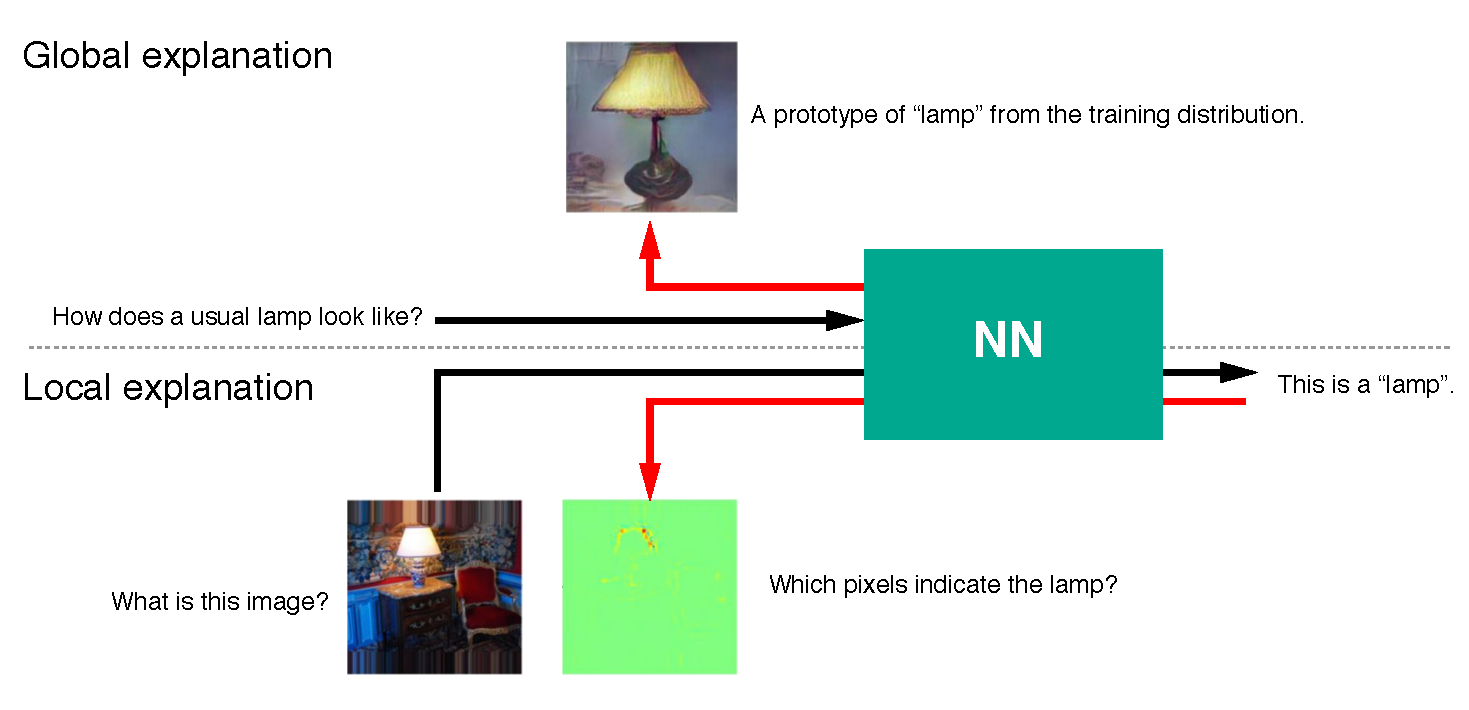
\includegraphics[width=0.8\textwidth]{sketch/global_and_local_method}
\caption{Comparison between global and local explanation}
\small{
The analogy is borrowed from Prof. M\"{u}ller's lecture slide. \\The images were taken from \cite{NguyenSynthesizingpreferredinputs2016a, BachPixelWiseExplanationsNonLinear2015}.
}
\label{fig:comparision_between_global_and_local_analysis}
\end{figure}

In the following, we are going to discuss approaches in local explanation in details and leave content of global explanation aside due to scope of the thesis. In particular, we are going to introduces these local explanation methods, namely \textit{sensitivity analysis}, \textit{guided backprop}, \textit{simple Taylor decomposition}, \textit{Layer-wise Relevance Propagation} and \textit{deep Taylor decomposition}.


%Consider $f(\patvector{x})$ is an output from a neural network classifier that is corresponding to the class prediction, for example the value at the final layer before applying softmax function.
%\begin{definition} Conservation Property
%\begin{align*}
%	\forall \patvector{x} : f(\patvector{x}) = \sum_i R_i
%\end{align*}
%Sum of relevance score of each pixel $x_i$ should equal to the total relevance that the network outputs.
%
%\end{definition}
%\begin{definition} Positivity Property
%\end{definition}
%\begin{definition} Consistency
%\end{definition}

\subsection{Sensitivity Analysis}
Sensitivity analysis(SA)\cite{SimonyanDeepConvolutionalNetworks2013} is a local explanation that derives relevance score $R_i(\x)$ through the  partial derivative of $f(\patvector{x})$ respect to $x_i$. In particular, it is formulated as follows 

\begin{align}
	R_i(\x) =
	 \bigg( \frac{\partial f(\patvector{x})}{ \partial x_i } \bigg)^2
\end{align}

which can then be interpreted as
\begin{align}
	\sum_i R_i(\x) = || \nabla f(\patvector{x}) ||^2
\end{align}

The derivation of $\sum_i R_i(\x)$ above implies that SA seeks to explain $R_i(\x)$ from the aspect of variation magnitudes of $f(\x)$, which might not reflect the actual influence of the pixels to the decision.

However, this technique can be easily implemented in modern deep learning frameworks, such as TensorFlow\cite{AbadiTensorFlowLargeScaleMachine2016}, via automatic differentiation. Hence, one might consider it to as a first tool towards explainability of neural networks.

\subsection{Guided Backpropagation}
Guided backpropagation(GB) is a extended version of sensitivity analysis where gradients are propagated throughout the network in a controlled manner. It is specifically designed for neural networks that use piecewise linear activations, such as ReLU. Formally, \cite{SpringenbergStrivingSimplicityAll2014e} proposed an alternative definition  of ReLU function as
\begin{align}
	\sigma(a_j) = a_j \mathbbm{1}[ a_j > 0 ],
\end{align}
where $\mathbbm{1}[ \cdot ]$  is an indicator function, and defined a new derivative of a ReLU neuron $j$ as:
\begin{align}
	\frac{\partial_* f(\patvector{x}) }{ \partial a_j } = \mathbbm{1}\bigg[a_j > 0 \bigg] \mathbbm{1}\bigg[ \frac{ \partial f(\patvector{x}) }{ \partial a_j } > 0 \bigg] \frac{ \partial f(\patvector{x}) }{ \partial a_j } 
\end{align}
From the derivation above, $\mathbbm{1}[ \cdot ]$ controls whether original gradients are propagated back, in particular, the gradients will be propagated to the previous layer only if neuron $j$ is active and the gradient from the next layer is positive. Similar to SA, the relevance score for each pixel is computed as 

\begin{align}
	R_i(\x) = \bigg( \frac{ \partial_* f(\patvector{x}) }{ \partial x_i }  \bigg)^2
\end{align}
%
%With this result, one can see that $x_i$ is relevant to the problem if activations $a_j$ that it supplies are active and positively contribute to $f(\patvector{x})$.

\subsection{Layer-wise Relevance Propagation}
The methods mentioned so far derive $R_i(\x)$ directly from $f(\patvector{x})$ and do not  use important knowledge about the network itself, such as architecture or activation values. Alternatively, Bach et	 al.\cite{BinderLayerWiseRelevancePropagation2016} propose Layer-wise Relevance Propagation(LRP) framework that leverages this known information to distribute relevance scores to $x_i$. In particular, LRP propagates relevance scores backward from layer to layer, similar to the back-propagation algorithm of gradient descent.




 \begin{figure}[!hbt]
	\begin{center}
		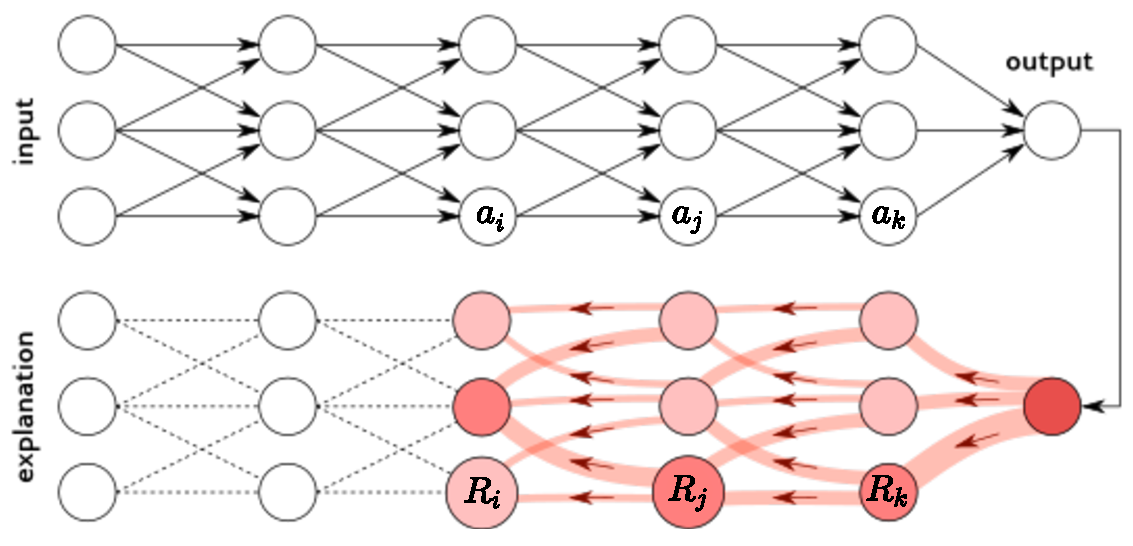
\includegraphics[width=0.8\textwidth]{sketch/lrp_graph}
		\caption{An illustration of relevance propagation in LRP.}
		\small{
			Source : \url{http://heatmapping.org}
			}
		\label{fig:lrp_graph}
	\end{center}
\end{figure}
%\footnotetext{}}
%}

Consider the neural network illustrated in \addfigure{\ref{fig:lrp_graph}}. $R_j$ and $R_k$ are relevance score of  neurons $j,k$ in successive layers.  LRP provides a general form of relevance propagation as 

\begin{align} \label{eq:general_lrp_rj}
	R_j = \sum_{k} 	\delta_{j\leftarrow k} R_{k} ,
\end{align}

where $\delta_{j\leftarrow k}$ defines a proportion that  $R_{k}$ contributes to $R_j$. Consider further that activity $a_k$ of neuron $k$ is computed by 
\begin{align}
	a_k = \sigma \bigg( \sum_{j} w_{jk} a_j + b_k \bigg),
\end{align} 
where $\sigma$ is a activation function, $w_{jk}, b_k$ are the corresponding weight and bias between neuron $j$ and $k$. For monotonic increasing $\sigma$, $\delta_{j\leftarrow k}$ can be calculated as follows 
\begin{align} \label{eq:delta_j_k}
	\delta_{j\leftarrow k} = \alpha\frac{a_j w_{jk}^+}{\sum_{j} a_jw_{jk}^+} - \beta\frac{a_j w_{jk}^-}{\sum_{j} a_jw_{jk}^-},
\end{align}
where $w_{jk}^+$, $w_{jk}^-$ are $\max(0, w_{jk})$, $\min(0, w_{jk})$, and $\alpha$,  $\beta$ are parameters with $\alpha-\beta = 1$ restriction. Combining (\ref{eq:general_lrp_rj}) and (\ref{eq:delta_j_k}) results in LRP-$\alpha\beta$ rule, 

\begin{align}
	R_j = \sum_{k} 	\bigg( \alpha\frac{a_j w_{jk}^+}{\sum_{j} a_jw_{jk}^+} - \beta\frac{a_j w_{jk}^-}{\sum_{j} a_jw_{jk}^-} \bigg )  R_{k}
\end{align}

Algorithm \ref{algo:lrp} summaries how LRP works.

\begin{algorithm}[H]
$f(\patvector{x}), \{ \{a\}_{l_1}, \{a\}_{l_2}, \dots, \{a\}_{l_n}\}$ = \text{forward\_pass}($\patvector{x}, \patvector{\theta}$)\;
$R_k = f(\patvector{x})$\;
 \For{ $\text{layer} \in \text{reverse}(\{l_1, l_2, \dots, l_n\})$}{
$ \text{prev\_layer} \leftarrow \text{layer}  - 1$ \;
	\For{ $j \in $ neurons(prev\_layer), $k \in$ neurons(layer)}{
		$R_j \leftarrow \text{LRP-}\alpha\beta(R_k, \{a\}_j, \{ w \}_{j,k} )$
	}
 }
 \caption{LRP Algorithm}
 \label{algo:lrp}
\end{algorithm}


Alternatively, if we slightly rearrange  the rule to 
$$
	R_j = \sum_{k} \bigg( \frac{a_j w_{jk}^+}{\sum_{j} a_jw_{jk}^+} \hat{R}_{k} + \frac{a_j w_{jk}^-}{\sum_{j} a_jw_{jk}^-} \check{R}_{k} \bigg),
$$ 
where $\hat{R}_{k}  = \alpha R_{k}$ and  $\check{R}_{k} = -\beta R_{k} $. We can then intuitively interpret this propagation as 

\begin{quote}
``Relevance $\hat{R}_k$'' should be redistributed to the lower-
layer neurons $\{a_j\}_j$ in proportion to their excitatory effect on $a_k$. ``Counter-relevance'' $\check{R}_k $ should be redistributed to the lower-layer neurons $\{a_j\}_j$ in proportion to their inhibitory effect on $a_j$
	- Section 5.1 \cite{MontavonMethodsInterpretingUnderstanding2017}
\end{quote} 

Moreover, LRP has \textit{Conservation Property} in which relevance quantities are conserved during distributing $f(\patvector{x})$ back to $\x$. Formally, it is 
\begin{align}
	\sum_{i} R_i =  \cdots =	\sum_{j} R_j = \sum_{k} R_k = \cdots = f(\patvector{x})
\end{align}


Nonetheless, choices of $\alpha,\beta$ is still a question for LRP.  In particular, \cite{MontavonMethodsInterpretingUnderstanding2017, BinderLayerWiseRelevancePropagation2016} demonstrated that the influence of the values to explanation heatmaps are depend on network architecture. For example, \cite{MontavonMethodsInterpretingUnderstanding2017} observed that LRP-${\alpha_1, \beta_0}$ works well for deep architectures, such as GoogleNet\cite{SzegedyGoingDeeperConvolutions2014}, while LRP-${\alpha_2, \beta_1}$ is better for shallower architectures, such as BVLC CaffeNet\cite{JiaCaffeConvolutionalArchitecture2014}.


%However, it seems that there is no clear relationship between values of $\alpha,\beta$ and the structure of the heatmap.  demonstrate that the values are depend on the architecture of the network. In particular, 
%




\subsection{Simple Taylor Decomposition}
As the name suggested,  the method decomposes $f(\patvector{x})$ using Taylor series around the root point $\tilde{\x}$ where the relevance scores $R_i(\x)$ are the first order terms of the series.

% into terms of relevance scores $R_i$ via Taylor decomposition. Formally, 

\begin{align} \label{eq:simple_taylor_expansion}
	f(\patvector{x}) 	&= f(\tilde{\patvector{x}}) + \sum_{i} \underbrace{\frac{\partial f }{ \partial x_i } \Bigg|_{x_i = \tilde{x}_i}  ( x_i - \tilde{x}_i ) }_{R_i} + \zeta, 
\end{align}
where $\zeta$ are the second and higher order terms that are not considered here. The root point $\tilde{\x}$ can be found via the optimization below 
\begin{align}
\underset{\xi \in \mathcal{X} }{\text{min}}  || \xi - \patvector{x} ||^2 \hspace{2cm}  \text{such that}\  f(\xi) = 0,
\end{align}

where $\mathcal{X}$ represents the input distribution. This optimization is time consuming  and $\xi$ might potentially be \todo{Check property : close to} or diverge from $\patvector{x}$ leading to non informative $R_i$. However, for neural networks using piecewise linear activations, such as ReLU,  $\tilde{\x}$ can be computed analytically. In particular, with assumptions of $\sigma(tx) = t\sigma(x) ,\forall t \ge 0$ and no use of bias, \cite{MontavonMethodsInterpretingUnderstanding2017} argued that $\tilde{\patvector{x}}$ can be found in  approximately the same flat region as $\patvector{x}$, $\tilde{\patvector{x}} = \underset{\epsilon \rightarrow 0 }{\lim} \epsilon \patvector{x}$, yielding

\begin{align}
	\frac{\partial f(\patvector{x})}{\partial x_i}\bigg|_{\patvector{x}={\tilde{\patvector{x}}}} = \frac{\partial f(\patvector{x})}{\partial x_i}\bigg|_{\patvector{x}={\patvector{x}}} 
\end{align}

%demonstrate that  neural networks whose activations $\sigma(x)$ are piecewise linear functions  with , for example a deep Rectified Linear Unit (ReLU) network without biases, 
%
As a result, (\ref{eq:simple_taylor_expansion}) can be simplified to :
\begin{align}
	f(\patvector{x}) &= \sum_{i} \frac{\partial f(\patvector{x})}{\partial x_i}\bigg|_{\patvector{x}={\patvector{x}}}  x_i \\
	R_i &= \frac{\partial f(\patvector{x})}{\partial x_i}\bigg|_{\patvector{x}={\patvector{x}}}  x_i \label{eq:simple_r_i}
\end{align} 

One can also interpret the relationship between sensitivity analysis and simple Taylor decomposition from (\ref{eq:simple_r_i}). Specifically, $x_i$ has high relevance score if $x_i$ highly activates and its variation positively affects $f(x)$ and vice versa.


%it is ensured that $$. Hence,  this decomposition can be simplified to :
%\begin{align*}
%	f(\patvector{x}) = 
%\end{align*}
%%

\subsection{Deep Taylor Decomposition}
Using Taylor decomposition as a foundation, deep Taylor decomposition(DTD) is a explanation technique that decomposes $R_k$ into Taylor series where $R_j$ from previous layer are the first order terms. \cite{MontavonExplainingnonlinearclassification2017} proposed the method to explain decisions of neural networks with piece-wise linear activations. Similar to LRP, DTD repeatedly decomposes relevances at the last layer $R_k$ and propagates the quantities to $R_j$ in the previous layer until the relevance of input pixel $R_i(\x)$. In particular, $R_k$ is decomposed as follows :


% In fact, it can be shown that LRP's propagation rule is equivalent to one of DT's rules.


 \begin{align} \label{eq:tl_rj}
 R_k = R_k \bigg|_{ \tilde{\patvector{a}}_j } + \sum_{ j } 	\frac{\partial  R_k }{ \partial a_j } \bigg|_{ a_j = \tilde{a}_j } ( a_j - \tilde{a}_j ) + \zeta_k
 \end{align}

Assume further that there exists a root point $\tilde{\patvector{a}}_j$ such that $R_k = 0$, and the second and higher terms $\zeta_k = 0 $. Then, (\ref{eq:tl_rj}) can be reduced to
\begin{align} \label{eq:R_k_sum}
 R_k = \sum_{ j } \underbrace{	\frac{\partial  R_k }{ \partial a_j } \bigg|_{ a_j = \tilde{a}_j }  ( a_j - \tilde{a}_j ) }_{ R_{j \leftarrow k } }
\end{align}

As the relevance propagated back,  $R_j$ is $\sum_{k} R_{j\leftarrow k}$ from neuron $k$ in the next layer that neuron $j$ contributes to. Hence, DTD has \textit{Conservation Property}, 
%Combining Equation \ref{eq:R_k_sum} and \ref{eq:R_j_sum} yields :
\begin{align} 
	R_j &= \sum_{k} R_{j\leftarrow k} \label{eq:rj_from_rk} \\
\sum_{j}	R_j &= \sum_{j} \sum_{k} R_{j\leftarrow k}\\
\sum_{j}	R_j &= \sum_{k} \sum_{j} R_{j\leftarrow k} \\
\sum_{j}	R_j &= \sum_{k}  R_{k} \\
\sum_i 	R_{i} = 	\dots = \sum_j R_{j} &= \sum_k R_{k} = \dots =  f(\patvector{x}) \label{eq:rj_equal_rk}
\end{align}

%Demonstrated by \cite{MontavonExplainingnonlinearclassification2017}, Equation \ref{eq:rj_equal_rk} holds for all $j, k$ and all subsequent layers. Hence, this results in  conservation property which guarantee that no relevance loss during the propagations.
%\begin{align}
%\sum_i 	R_{i} = 	\dots = \sum_j R_{j} = \sum_k R_{k} = \dots =  f(\patvector{x})
%\end{align}
 
 
%\begin{figure}[h]
%\centering
%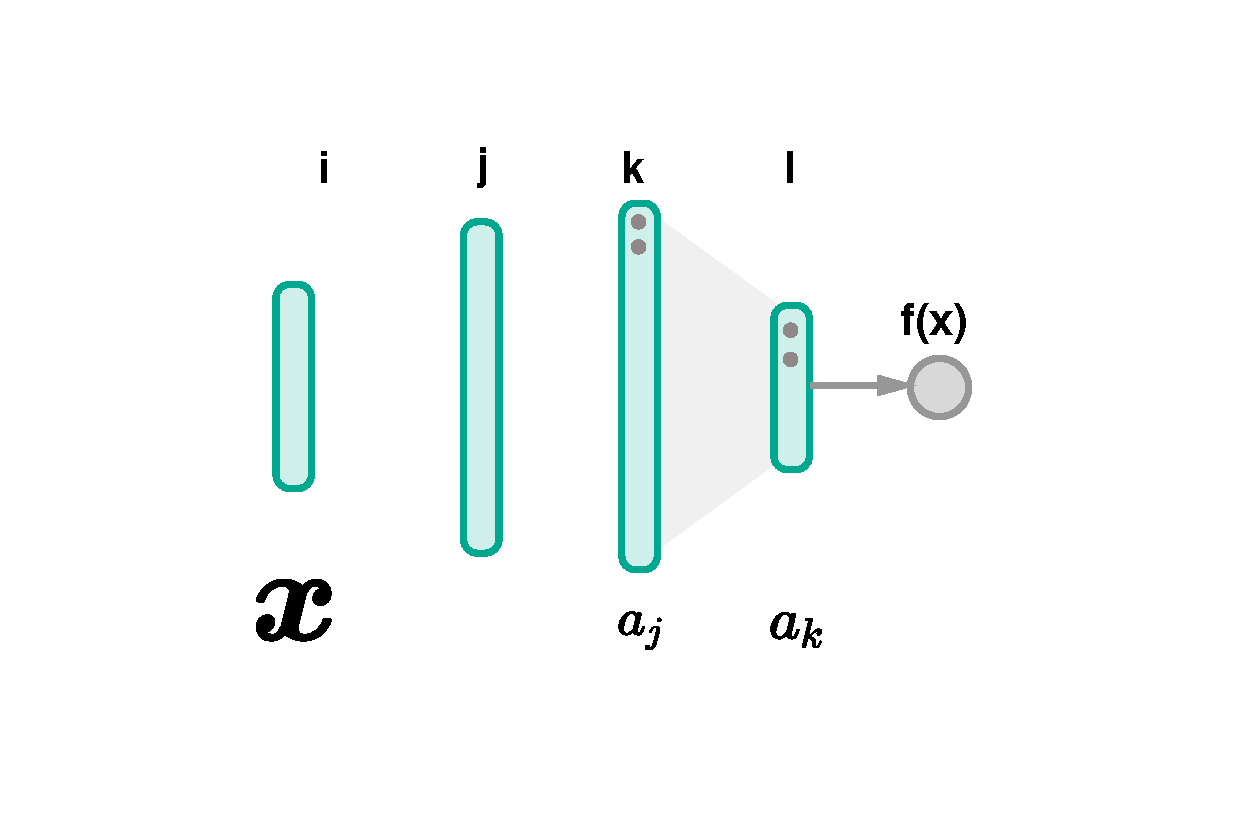
\includegraphics[width=0.8\textwidth]{sketch/deep_tayloy_decomposition_toy}
%\caption{A Simple network}
%\label{fig:deep_tayloy_decomposition_toy}
%\end{figure}

\subsubsection{Finding the root point}
Consider a neural network whose $R_k$ is based on activations of $a_j$ in the previous layer and computed by :
\begin{align}\label{eq:r_k_deep_taylor}
R_k = \text{max}\ \bigg(0, \sum_{j} a_j w_{jk}  + b_k \bigg),
\end{align}
where $b_k \le 0 $.

To find the root point $\tilde{\patvector{a}}_j$, one can see that  there are  2 cases to be analyzed, namely $R_k = 0$ and $R_k > 0$. For $R_k=0$,  $\patvector{a}_j$ is already the root point. For the latter, the root point can be found by performing  line search in  some direction $\patvector{v}_j$ and magnitude $t$.
\begin{align}\label{eq:root_aj_aj}
\tilde{a}_j = a_j - t v_j,
\end{align}
More precisely, the root point is the intersection point between (\ref{eq:r_k_deep_taylor}) and (\ref{eq:root_aj_aj}) where $R_k=0$. Hence,
\begin{align}
  0 &= 	\sum_{j} (a_j - t v_j) w_{jk}  + b_k\\
%  0 &= \sum_{j} a_j w_{jk} - t v_j w_{jk}  + b_k\\
  t \sum_{j} v_j w_{jk} &= R_k \\
  t &= \frac{R_k}{\sum_{j} v_j w_{jk}}
\end{align}

Combining
Therefore, $R_j$ can be computed by :
\begin{align}
R_j &= \sum_k	\frac{\partial  R_k }{ \partial a_j } \bigg|_{ a_j - \tilde{a}_j }  ( a_j - \tilde{a}_j ) \\
&=	\sum_k w_{jk} tv_j \\
&=	\sum_k \frac{ v_j w_{jk}   }{\sum_{j} v_j w_{jk}}  R_k
\end{align}

\begin{figure}[!hbt]
\centering
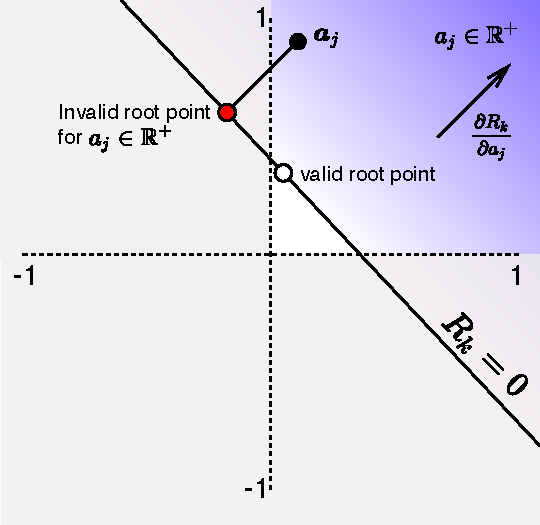
\includegraphics[width=0.4\textwidth]{sketch/invalid_root_point_example}
\caption{Function's view of $R_k$  and root point candidates}
\label{fig:root_point_illus}
\end{figure}



The last step is to find $\boldsymbol{v}_j$ such that $\tilde{\patvector{a}}_j$ is the closest point in the same domain as $\patvector{a}_j$ to the line $R_k=0$. \addfigure{\ref{fig:root_point_illus}} visualizes the intuition. Here, if $a_j \in \mathbb{R}^+$, then $\tilde{a}_j$ must be also in $\mathbb{R}^+$. Therefore, $\boldsymbol{v}_j$ needs to be separatedly derived for each possible domain.
% of $\patvector{a}_j$.

%Noticing here is that $\tilde{\patvector{a}}_j$ is not necessary the closest point to the line $R_k=0$ in Euclidean distance, because  $\tilde{\patvector{a}}_j$  might not be in the same domain as $\patvector{a}_j$, hence $v_j$ needs to be chosen according to the domain of $\patvector{a}_j$. Consider an example on \addfigure{\ref{fig:root_point_illus}}, if $a_j \in \mathbb{R}^+$, then $\widetilde{a_j}$ must be also in $\mathbb{R}^+$.   In the following, I will summarize how $\patvector{a}_j$ can be computed for each domain of $\patvector{a}_j$.

\subsubsection{Case $a_j \in \mathbb{R}$ : $w^2$-rule}

Trivially, the search direction $v_j$ is just the direction of gradient $\frac{\partial  R_k^{(l+1)} }{ \partial a_j^{(l)} }$:
\begin{align*}
	v_j = w_{jk}
\end{align*}

Hence, 
\begin{align*}
	R_j &=	\sum_k \frac{ w_{jk}^2  }{\sum_{j} w_{jk}^2}  R_k
\end{align*}

\subsubsection{Case $a_j \in \mathbb{R}^+$ : $z^+$-rule}
\begin{figure}[!htb]
\centering
\subfloat[]{%
       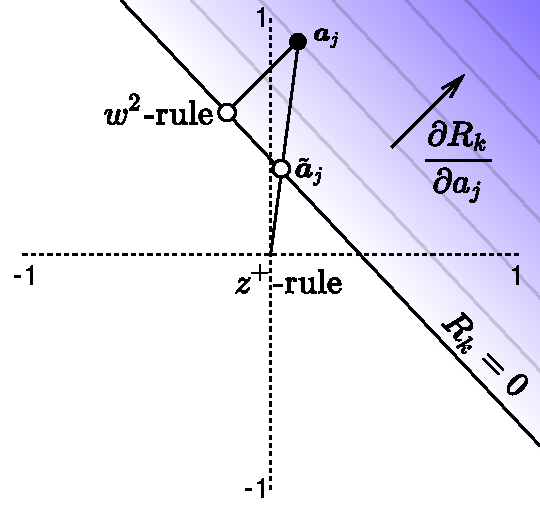
\includegraphics[width=0.4\textwidth]{sketch/zplus_rule_case_1}
     }
%     \hfill
     \subfloat[]{%
       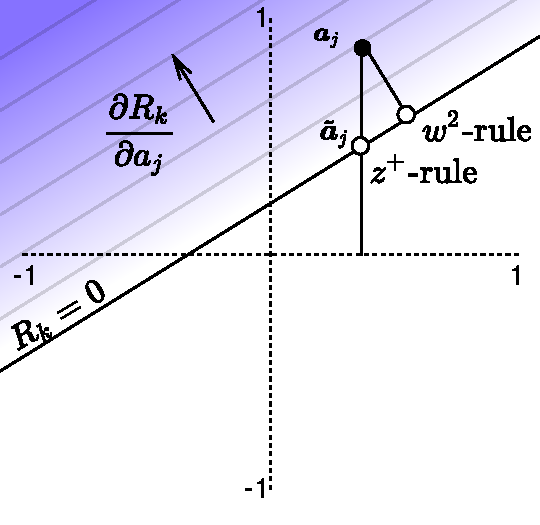
\includegraphics[width=0.4\textwidth]{sketch/zplus_rule_case_2}
     }
\caption{Function's view of $R_k$ and the root point from $z^+$-rule}
\label{fig:zplus_rule_cases}
\end{figure}

The root point is on the line segment $( a_j \mathbbm{1}[ w_{jk}  < 0 ], a_j )$. In particular, as shown on \addfigure{\ref{fig:zplus_rule_cases}}, $R_k$ has a root at $a_j \mathbbm{1}[w_{jk}  < 0 ]$, because of:
\begin{align}	
R_k &= \max \bigg( \sum_j a_j w_{jk } + b_k, 0 \bigg) \\
&=  \max \bigg( \sum_j a_j \mathbbm{1}[ w_{jk}  < 0 ] w_{jk} + b_k, 0 \bigg) \\
&=  \max \bigg(\sum_j a_j  w_{jk}^- + b_k , 0\bigg) \\
&= 0 \label{eq:zplus_rk_zero}
\end{align}
The last step uses the fact that $a_j \in R^+$ and $b_k \le 0$ from the assumption. Hence, the search direction is:
\begin{align}
	v_j &= a_j - a_j \mathbbm{1}[ w_{jk}  < 0 ] \\
	&= a_j \mathbbm{1}[ w_{jk}  \ge 0 ]
\end{align}




Therefore, 
\begin{align}
		R_j &=	\sum_k \frac{ w_{jk} a_j \mathbbm{1}[w_{jk}  \ge 0 ]  }{\sum_{j} w_{jk} a_j \mathbbm{1}[ w_{jk}  \ge 0 ]}  R_k\\
		&=	\sum_k  \frac{ a_j  w_{jk}^+   }{\sum_{j}  a_j w_{jk}^+  }  R_k
\end{align}

This results the propagation rule that  is equivalent to LRP-$\alpha_1\beta_0$. 


\subsubsection{Case $a_j \in [l_j , h_j]$ where $l_j \le 0 < h_j $ : $z^\beta$-rule}

\begin{figure}[!htb]
\centering
\subfloat[]{%
       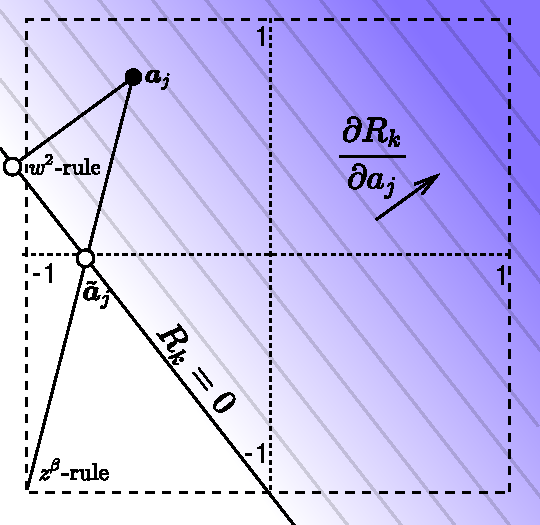
\includegraphics[width=0.4\textwidth]{sketch/zbeta_rule_case_1}
     }
%     \hfill
     \subfloat[]{%
       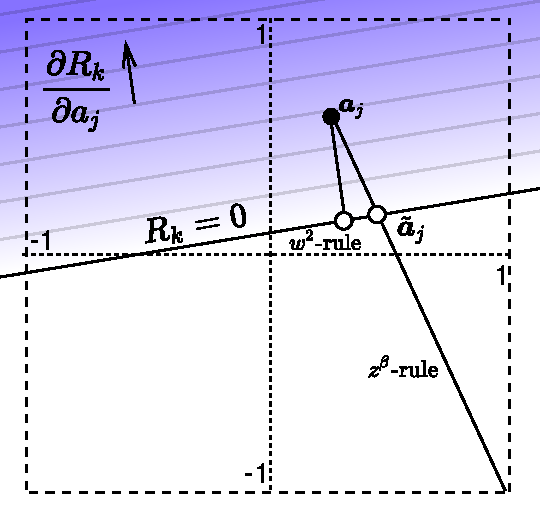
\includegraphics[width=0.4\textwidth]{sketch/zbeta_rule_case_2}
     }
\caption{Function's view of $R_k$ and the root point from $z^\beta$-rule with $-1 < a_j < 1$ }
\label{fig:zbeta_rule_cases}
\end{figure}
This situation associates to the first layer where the input is bounded, for example pixel intensity. In this case, as shown in \addfigure{\ref{fig:zbeta_rule_cases}}, the root point is on the line segment $( l_j \mathbbm{1}[ w_{jk}  \ge 0 ]  + h_j \mathbbm{1}[ w_{jk}  \le 0 ]  , a_j ) $. In particular, the root point is at $l_j \mathbbm{1}[ w_{jk}  \ge 0 ]  + h_j \mathbbm{1}[ w_{jk}  \le 0 ]$,
\begin{align}
R_k &= \max \bigg( \sum_j a_j w_{jk } + b_k, 0 \bigg) \\
&=\max \bigg( \sum_j (l_j \mathbbm{1}[ w_{jk}  \ge 0 ]  + h_j \mathbbm{1}[ w_{jk}  \le 0 ] ) w_{jk } + b_k, 0 \bigg) \\
&= \max \bigg( \sum_j l_j w_{jk }^+   + h_j w_{jk }^-  + b_k, 0 \bigg) \\
&= 0
\end{align}

Hence,  the search direction is 
\begin{align}
	v_j &= a_j - \tilde{a}_j \\
	&=a_j  - l_j \mathbbm{1}[ w_{jk}  \ge 0 ]  - h_j \mathbbm{1}[ w_{jk}  \le 0 ]
\end{align}

Therefore, 
\begin{align}
		R_j &=	\sum_k \frac{ w_{jk}  (a_j  - l_j \mathbbm{1}[ w_{jk}  \ge 0 ]  - h_j \mathbbm{1}[ w_{jk}  \le 0 ]) }{\sum_{j} w_{jk}  (a_j  - l_j \mathbbm{1}[ w_{jk}  \ge 0 ] - h_j \mathbbm{1}[ w_{jk}  \le 0 ]) }  R_k\\
		&=	\sum_k  \frac{ a_j  w_{jk} - l_j w_{jk}^- - h_j w_{jk}^+  }{\sum_{j}   a_j  w_{jk} - l_j w_{jk}^- - h_j w_{jk}^+  -}  R_k
\end{align}





%In summary, DTD is a theory for explaining nonlinear compuations of neural network through decomposing relevance score between successive layers. Its propagation rules ensures conservation property. Given the rules above, the relevance scores can be propagated using LRP Algorithm \ref{algo:lrp}.
%
%Lastly, as DTD provides more general propagation rules than the $\alpha\beta$-rule from LRP, I will use DTD and LRP interchangeably throughout the thesis. In particular, it will be mentioned explicitly if $\alpha\beta$ is being used, otherwise the rule is a DTD's rule.  

Table \ref{tab:lrp_deep_taylor_rules} concludes the details  when each DTD rule should be applied. As a result, the relevance scores, $f(\x)$, can be propagated through the nextwork using LRP Algorithm \ref{algo:lrp}.


\renewcommand{\arraystretch}{1}
\begin{table}[h]
\centering
\begin{tabular}{|l|l|}
\hline
\multicolumn{1}{|c|}{Rule and input domain} & \multicolumn{1}{c|}{Formula} \\ \hline
$w^2$-rule : Real values,  $a_j \in \mathbb{R}$ & \parbox{1cm}{
	\begin{align*}
		R_j =	\sum_k \frac{ w_{jk}^2  }{\sum_{j} w_{jk}^2}  R_k  	
    \end{align*}}
 \\ \hline
% &                                \\ \hline
$z^+$-rule : ReLU activations, $a_j \in \mathbb{R}^+$    & \parbox{1cm}{\begin{align*}
R_j = \sum_k  \frac{ a_j  w_{jk}^+   }{\sum_{j}  a_j w_{jk}^+  }  R_k	
\end{align*}} \\ \hline
$z^\beta$-rule : Pixel Intensities, $ a_j \in [l_j , h_j]$ where $l_j \le 0 < h_j $  & \parbox{1cm}{\begin{align*}
R_j = \sum_k  \frac{ a_j  w_{jk} - l_j w_{jk}^- - h_j w_{jk}^+  }{\sum_{j}   a_j  w_{jk} - l_j w_{jk}^- - h_j w_{jk}^+  -}  R_k	
\end{align*}}
               \\ \hline
\end{tabular}
\caption{Relevance propagation rules of deep Taylor decomposition. }
\label{tab:lrp_deep_taylor_rules}
\end{table}
\renewcommand{\arraystretch}{1}


\begin{figure}[!htb]
\centering
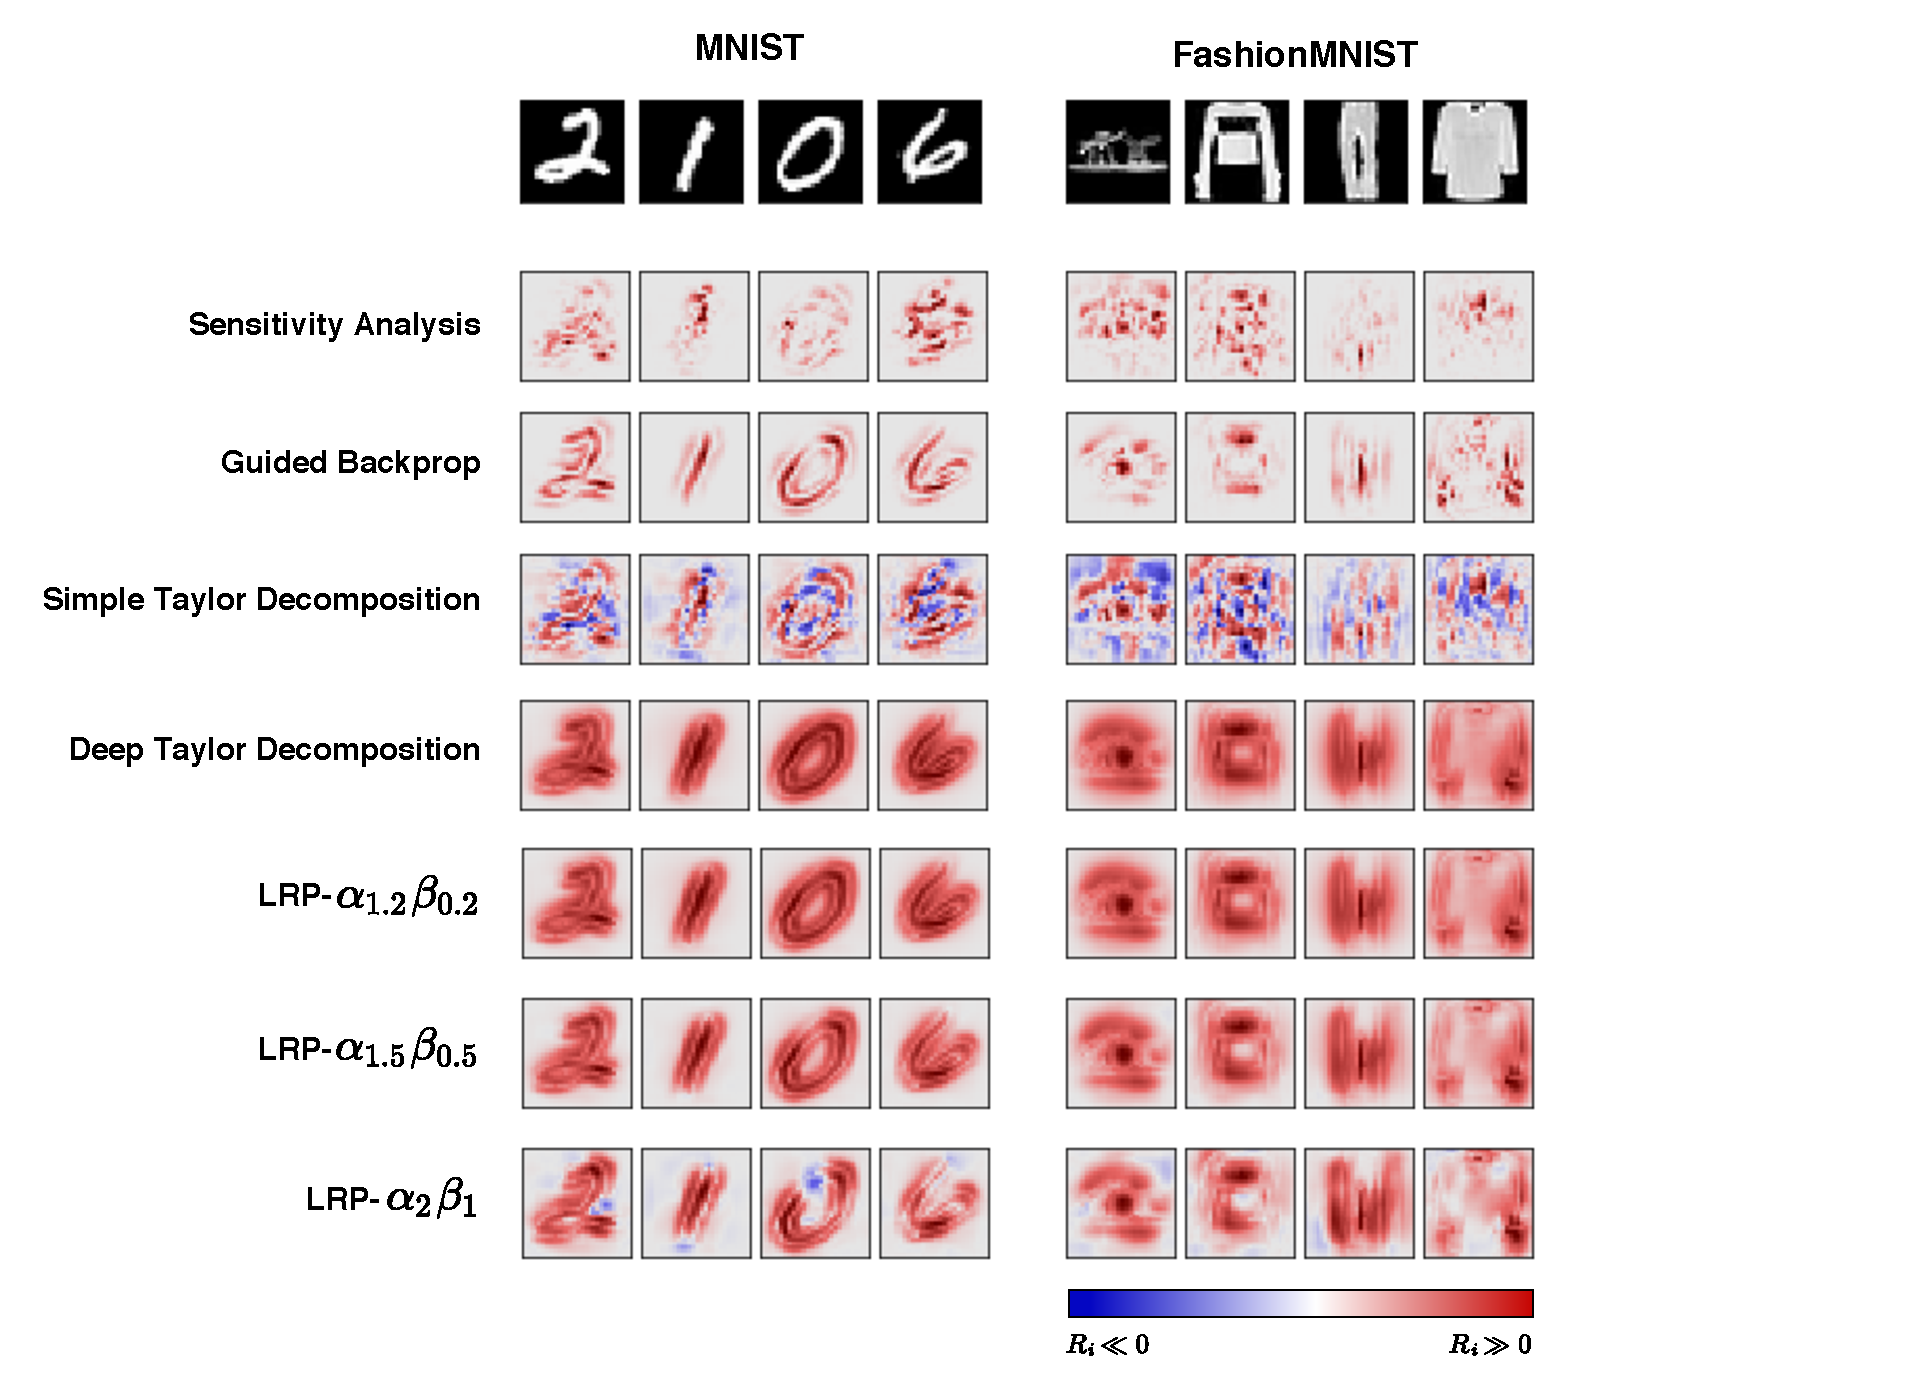
\includegraphics[width=\textwidth]{sketch/lenet_heatmaps}
\patcaption{Relevance heatmaps from LeNet-5 architecture explained by different explanation methods.}{\heatmapscaleexplain }
\label{fig:lenet_heatmaps}
\end{figure}

In this section, we have described several explanation methods as well as their intuition.  \addfigure{\ref{fig:lenet_heatmaps}} shows  examples of relevance heatmaps from those methods applied on LeNet-5\cite{LeCunGradientBasedLearningApplied2001} to explain classification decisions that the network makes. The network was trained on 100 epochs with batch size 50 and dropout probability at 0.2. It achieves accuracy at 99.21\% for MNIST and 87.90\% for FashionMNIST. From the figure, we can also see characteristics of each method. In particular, one can observe that simple Taylor decomposition provides the most noisy and non informative heatmaps, while explanations from sensitivity analysis(SA) also looks noisy but input features can be seen. Guided backprop(GB) produces smoother version of SA heatmaps. On the other hand, explanations from deep Taylor decomposition(DTD) and LRP are more diffuse and smoother than the others : they also look similar when $\beta$ is small.  Given this result, we are going to consider only SA, GB, DTD and $\lrpp$ in experiments.

	